\documentclass[a4paper,11pt,oneside,fleqn]{article}
% Pakker
\usepackage[utf8]{inputenc} % Så må vi bruge æ, ø og å
%\usepackage(ansinew){inputenc}
%\usepackage(danish){babel} % Dansk opsætning
\usepackage[T1]{fontenc} % Hjælper med orddeling ved æ, ø og å. Sætter fontene til at være ps-fonte i stedet for bmp.
\usepackage[english,final]{varioref} % Vi kan anvende \vref
\usepackage{array,booktabs} % Til gode tabeller
\usepackage[printonlyused,withpage]{acronym} % Smart akronymhåndtering
\usepackage{minitoc} % Vi kan lave del inholdsfortegnelser forhåbentlig
\usepackage{graphicx} % We can now use \includegraphics and stuff
\usepackage[svgnames]{xcolor} % Colored stuff i.e. \colorbox
\usepackage{pdfpages} % Inkludere en pdf side som en side  
\usepackage{amsmath,amsfonts,amssymb} % God matematik
\usepackage{wasysym}% smileys
\usepackage{textcomp} % More text stuff, such as numero
\usepackage{mathtools} % We can now use \xRightarrow{hello world}
\usepackage{booktabs} % Rulers for tables
\usepackage[thinspace,amssymb]{SIunits} % Using macros for typesetting SI units
\usepackage{natbib} % Use proper citation
\usepackage{tocbibind} % Includes toc and bib in toc
\usepackage{listingsutf8} % Code listings
\usepackage{tabularx,booktabs} % Tables with fixed width
\usepackage{todonotes} % Todonotes
\usepackage{tcolorbox} % Colored boxes!
\lstset{extendedchars=\true, inputencoding=utf8/latin1} % This and listingsutf8 makes us able to use utf8 and latin1 as inputfiles
\lstset{language=matlab,frame=single,basicstyle=\footnotesize\ttfamily}
\usepackage[pdftex]{hyperref} % Hyperlinks
\hypersetup{backref,
bookmarks=true,
bookmarksnumbered=true,
colorlinks=true,
linkcolor=Navy,
citecolor=Green} % Setting some fancy colors
\DeclareUnicodeCharacter{00A0}{~} % Fix odd OSX/textwrangler no break space charater
\newcommand{\head}[1]{\vspace{3mm}{\noindent \hspace{-0.5em} \fcolorbox{gray}{GhostWhite}{\parbox[c]{\textwidth}{\slshape{#1}}}\vspace{2mm}}} % Header

\let\oldhat\hat
\renewcommand{\vec}[1]{\boldsymbol{#1}}
\renewcommand{\hat}[1]{\oldhat{\mathbf{#1}}}

\newcommand{\MATLAB}{M{\footnotesize ATLAB}}

\begin{document}
% Frontpage
\author{Nick Østergaard}
\title{Users Manual\\
	for\\
\emph{ASV Formation Control for Surveying Purposes}}
\date{\today}
\maketitle
\thispagestyle{empty}
\begin{center}
	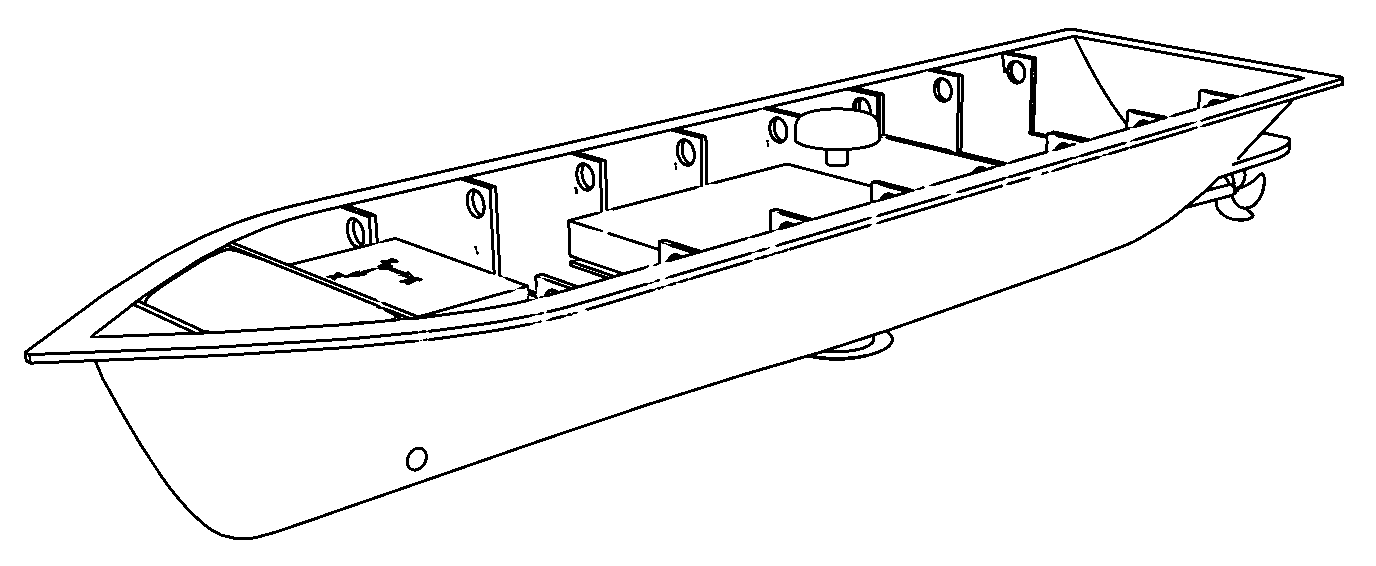
\includegraphics[width=13cm]{fig/aauship}
\end{center}
\vfill
\begin{center}
	
\includegraphics[width=5cm]{fig/AAU_LOGO_CMYK_UK}\\
	Department of Electronic Systems
\end{center}
\clearpage

% Abstract
\begin{abstract}\addcontentsline{toc}{section}{Abstract}

This report documents the design and implementation of optimal control
of a helicopter test setup controlling the travel and elevation with
and without feedback using a linear quadratic controller.

The helicopter model has 3 degrees of freedom, controlled by two
horizontal propellers to adjust pitch and elevation, nonzero pitch
makes it travel.

The implementation is done in \MATLAB\ and with QuaRC from Quanser
integrated with Simulink and MathWorks' Real-Time Workshop. The code
and simulink models are also presented in the appendix.
	
\end{abstract}


% Table of contents
\tableofcontents
%\listoftables
%\listoffigures
\newpage

% Inclusion of body text here
\chapter{Introduction}
\head{In this chapter is the motivation for the project stated and the previous work within the subject will be summed up.}

\section{Motivation and the AAUSHIP Project}
The Port of Aalborg would like Aalborg University to help them to expand their options of improving the conditions of the Limfjord. One of their tasks is to map the seabed of the Limfjord to get bathymetry data. This will help them guide larger cargo ships to port while using the autonomous ships as guidance.

Another aspect from The Port of Aalborg is a task to escort larger ships with cargo into The Port of Aalborg. This is done by a pilot whom needs to sail out to incoming larger cargo ships and escort them safely into port. The pilot does this in a pilot boat which is controlled manually by the pilot. The Port of Aalborg would like this process to become autonomous such that an autonomous boat can sail to the cargo ship and to some extend take over the control and guide the cargo ship into port. The system to do this implies that The Port of Aalborg needs an autonomous ship which can perform this task.

The mapping itself can be done by one ship or by more. For the moment one of the ships from The Port of Aalborg, which is manned, and covers the mapping of the closer part of the Limfjord ($\approx$ 65 km). This is only done every third year, but mapping around Hals Barre (a sandbar \todo{slet efterfølgende kommentar igen engang}and not a beach bar) at the end of the Limfjord is a more critical place and is mapped every third month.

If The Port of Aalborg had an autonomous ship fleet at their disposal, which could sail out and do the mapping autonomously, they would get updated bathymetry maps with a higher update frequency than they have currently \citep{portofaalborg}. This will result in a digitalizing of the seabed, a digital map, which has different implementation options by The Port of Aalborg.

This thesis will utilise formation control and extensions to manoeuvre agents through a specified area for surveying purposes. The aspect of formation control is chosen due to the rather large areas that The Port of Aalborg needs so cover. When applying formation control it is assumed to be faster to cover a larger area than if one single boat needed to scan the area. The formation that are to be chosen depends on the specific area of interest, which could e.g. be inside the harbour or around the pillars of the bridge. Chapter~\vref{ch:formcontrol} will introduce what kind and scopes of formation control that exists today. These theories makes the basis for the formation control within the scope of this project.

As a future scope this can be used when making a model of the seabed of how this will get sanded. This model can tell The Port of Aalborg when to go clean the seabed. The AAUSHIP project can be used to verify this model, such that The Port of Aalborg do not have to go out with equipment to solve the sanding without the need of it.

\section{The Mission}
\label{sc:mission}
Within the scope of this project the robots will be unmanned ships,
\ac{ASV}. The ship's main purpose will be to map the seabed by using
sonars to obtain bathymetry data. When one ship need to do this alone, and due to the range of
the sonar, the time spend could be improved by using multiple ships. The sonar scanning would
be done as seen on figure~\vref{fig:concept-art}.

\begin{figure}[htbp]
	\centering
	\subfloat[One ship\label{fig:concept-art1}]{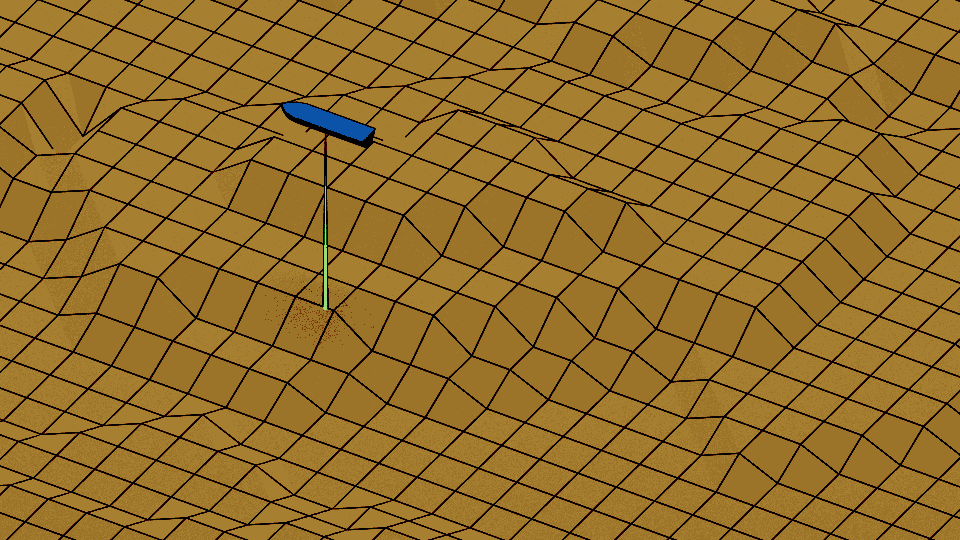
\includegraphics[width=0.48\textwidth]{fig/conseptart-single}}
	\ % One forced space to seperate figures
	\subfloat[Thee ships\label{fig:concept-art3}]{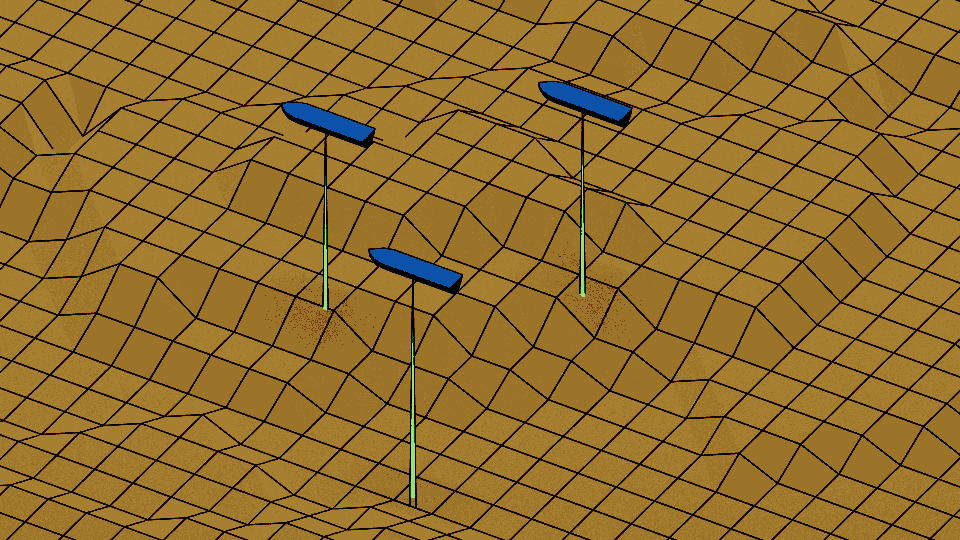
\includegraphics[width=0.48\textwidth]{fig/conseptart-formation}}
	\caption{Comparison of two ways to cover an area with a lawn mower
	pattern.}
	\label{fig:concept-art}
\end{figure}

When only one ship (figure~\vref{fig:concept-art1}) need to map a complete seabed this process could
take up much time dependent on the area that need to be covered. The
time spend could be improved to make this mapping more efficient. One
way of optimizing the time used is to add more ships (figure~\vref{fig:concept-art3}) to help map the
seabed. To make the process of this as optimal as possible it could be
of benefit to implement formation control in the specific assignment.

I cooperation with the port of Aalborg, a use case is presented, where we can perform tests of the platform, and use those to compare the performance of our system to their system.
\begin{figure}[htbp]
	\centering
	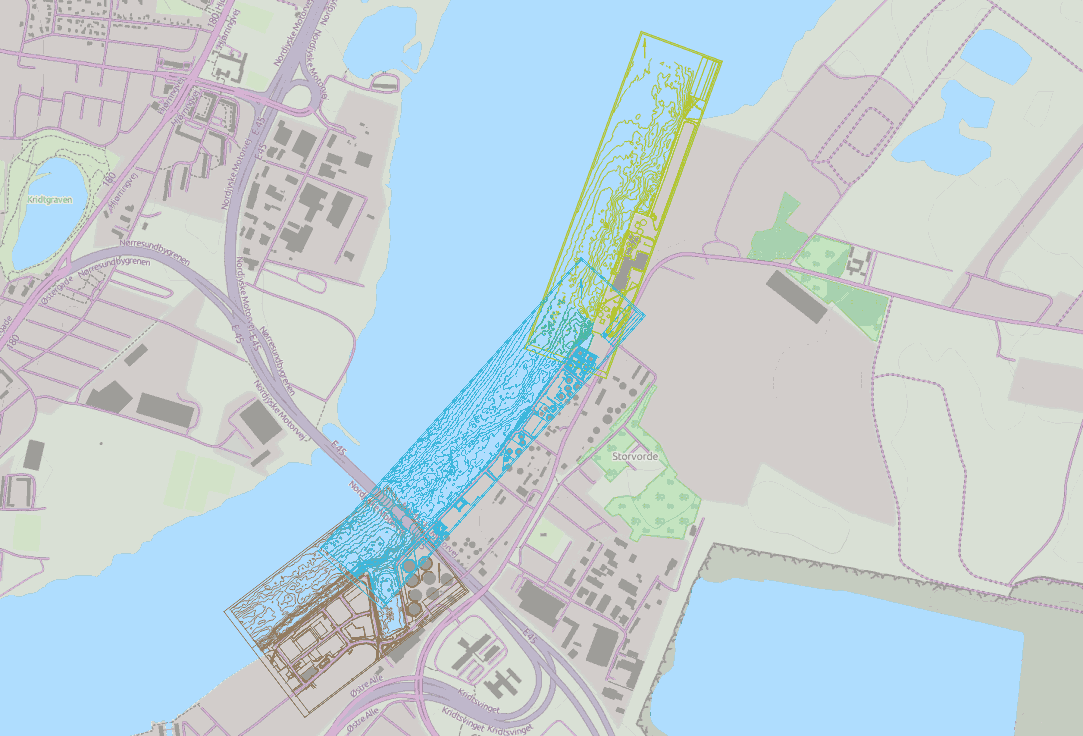
\includegraphics[width=\textwidth]{fig/use-case-data}
	\caption{Area of the harbour at Aalborg Portland provided as sample
	data from Aalborg Havn. Background map data CC BY-SA OpenStreetMap.}
	\label{fig:diffforms}
\end{figure}

When performing this kind of surveying with multiple ships, it is important to take note of the kind of sensor it uses and the coverage that it provides. Initially the port of Aalborg used single beam echo sounders, but have in recent years turned over to multibeam sonars for their survey boat, which has improved their resolution and time for a survey. But they still wishes to improve the survey update rate, by e.g. using fairly low cost autonomous ships to get better indication of the seabed to identify if an expensive thorough survey is needed. An image of the survey vessel they use now used can be seen on figure \ref{fig:alba}. As it can be seen, this survey vessel is relatively large, being over 20 metres long. To comparison is the AAUSHIP only 1.1 metres long. For surveying in smaller areas, like inside the harbour area, Aalborg Havn uses a smaller scale vessel which is 12 metres long. This vessel is only used at the smaller areas thus not the one being used out in the Limfjord close to Aalborg.
\begin{figure}
	\centering
	\includesvg{alba}
	\caption{The survey vessel used by Aalborg Havn named Alba.}
	\label{fig:alba}
\end{figure}



%This could be done in several ways, but is mostly thought of in a
%rigid formation, such that the formation maps the same area of the
%seabed the whole time. The idea can be seen on
%figure~\vref{fig:concept-art}.

\section{Objective}

\head{This section describes what can be done for humanity by the use of
automation in the realm of Aalborg.}

A use case that is a basis of this project is a service that surveying
companies offer, which is to survey and map the seabed of waterways and
lakes. Currently they do this very manually my sailing with a boat in
the lake after a \ac{GNSS} in the boat. In waterways as small rivers
and the like in Denmark they do it by a smaller boat or raft, where
they are using a prism system and a stick to take point measurements
of the river.

These tasks could be automated and probably improve surveying time by
using an autonomous system that can cover this. Here focus is on
trying to design such a system with small ships sailing in formation
to scan a predefined area.

This will then lead to defining the needed capabilities for
the formation control.

\todo{See 3.3.2 in \citep{thorvaldsen} for some nice definitions.}

\section{Parts list}
See table~\vref{tab:parts}.
\begin{table}[htbp]
	\centering
	\begin{tabularx}{\textwidth}{ll}
	\toprule
	\# &  Model \\
	\midrule
	2 & Graupner InIine 750 \\
	2 & Electronic Speed Controller \\
	2 & Propellers \\
	2 & Prop Shaft \\
	2 & Motor to prop shaft couplings 5mm\\
	6 & LiPo 3600 mAh 4S1P batteries \\
	1 & Intelligent Charge Port (ICP) \\
	1 & Raspberry Pi or similar \\
	1 & 4-split USB hub\\
	1 & Echosounder \\
	\bottomrule
	\end{tabularx}
	\caption{Mechanical parts for an AAUSHIP}
    \label{tab:parts}
\end{table}


\section{Power System}

The power source in AAUSHIP is chosen to be LiPo batteries, which is
a type of battery chemistry where the operator take great care in not damaging
the batteries. If care is not taken they might catch on fire, which
cannot easily be extinguished. This can of course be dangerous.

\subsection{Power Harness}
The power system on the ship consists of some somewhat convoluted
wiring harnessed loosely in the hull structures. An single line
diagram is therefor provided to give an overview of the system.

\begin{figure}[htbp]
	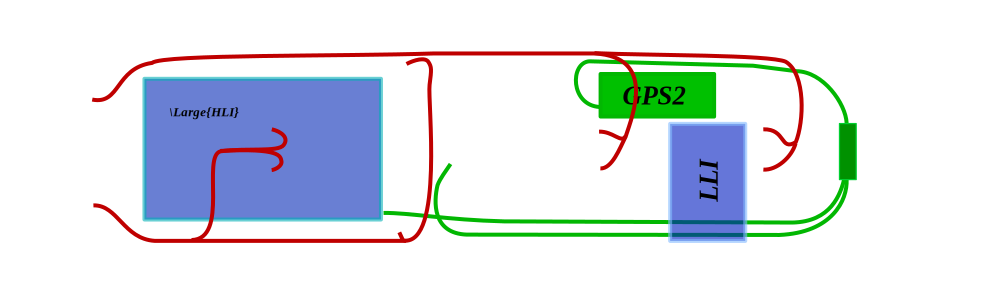
\includegraphics[width=\textwidth]{fig/harness}
\end{figure}

\subsection{LiPo Basics}
The LiPo battery packs each consists of four cells in series, which in
the LiPo battery world is called ``4S1P''. One parallel is what you get
when you only have a series connection.

Since each cell is normally not charged individually but across the
output terminals of the battery, every pack with more than one series
cell is equipped with a so called balance port. This is basically a
smaller multiple pin connector that has a connection to each cell,
such that is is possible for a ``balancer'' to discharge cells that is
unbalanced. An unbalanced cell is basically just a cell that does not
have the same voltage as the others.

This balancer is usually run whilst one is charging the main
connections. The purpose is to eliminate the difference that is
inherent in each cell not being exactly the same, such that one cell
does not get overcharged, when charging them in series.

\subsection{LiPo Battery Safety}
\begin{tcolorbox}[colback=yellow!75!,colframe=red]
It is strongly advised not to mess with the LiPo batteries before you
have read and understand how to handle them. A good resource for
learning some basics and safety about LiPo batteries are
\citep{tjintech:lipo-basics} and \citep{tjintech:lipo-safety}.
\end{tcolorbox}
 

\appendix
\chapter{Acronyms}
\label{ch:acronyms}
\begin{acronym}[TDMA]
%\begin{acronym}[HBCI]
	\acro{AAU}{Aalborg University}
  \acro{ASV}{Autonomous Surface Vessel}
	\acro{ADC}{Analog to Digital Converter}
  \acro{AHRS}{Attitude and Heading Reference System}
  \acro{BODY}{The body frame}
  \acro{CFD}{Computational Fluid Dynamics}
  \acro{DOF}{Degrees-Of-Freedom}
  \acro{DP}{Dynamic Positioning}
  \acro{ECEF}{Earth-Centered Earth-Fixed} 
  \acro{ECI}{Earth-Centered Inertial}
  \acro{EKF}{Extended Kalman Filter}
  \acro{FRF}{Formation Reference Frame}
  \acro{FRP}{Formation Reference Point}
	\acro{GNC}{Guidance, Navigation and Control}
  \acro{GNSS}{Global Navigation Satellite System}
  \acro{GPS}{Global Positioning System}
  \acro{GRS}{Ground Segment}
  \acro{HLI}{High Level Interface}
  \acro{IMU}{Inertial Measurement Unit}
	\acro{IP}{Internet Protocol}
	\acro{IPv4}{Internet Protocol version 4}
	\acro{IPv6}{Internet Protocol version 6}
  \acro{KF}{Kalman Filter}
  \acro{LKF}{Linear Kalman Filter}
  \acro{LOS}{Line-Of-Sight}
  \acro{LLI}{Low Level Interface}
	\acro{LSB}{Least Significant Bit}
  \acro{LTI}{Linear Time Invariant}
  \acro{MARG}{Magnetic, Angular Rate, and Gravity}
  \acro{MMSE}{Minimum Mean Square Error}
  \acro{MUV}{Multiple Unmanned Vehicle}
  \acro{MPC}{Model Predictive Control}
  \acro{NED}{North-East-Down}
  \acro{OSM}{OpenStreetMap}
  \acro{PWM}{Pulse Width Modulation}
  \acro{ROS}{Robot Operating System}
  \acro{RTK}{Real Time Kinematic}
  \acro{SOG}{Speed Over Ground}
  \acro{SSS}{Single Screw Ship}
  \acro{SSM}{State Space Model}
  \acro{TSS}{Twin Screw Ship}
  \acro{UGAS}{Uniformly Globally Asymptotically Stable}
  \acro{UGES}{Uniformly Globally Exponentially Stable}
  \acro{UGS}{Uniformly Globally Stable}
  \acro{UKF}{Unscented Kalman Filter}
  \acro{WGS84}{World Geodetic System 1984}
\end{acronym}



% Bibliography
%\bibliographystyle{apalike}
\bibliographystyle{plain}
\bibliography{bib}\label{sec:bibliography}

\end{document}
